\chapter{Light Matter Interaction}
\section{Basic of laser processing} %410

When dealing with laser processing, we will make the assumptions of steady state and spherical heat distribution.

\subsection{Heat conduction}
Heat conduction through a spherical shell is given by \ref{eq:hcss}.
\begin{equation}
    Q = -k (4 \pi r^2)\frac{dT}{dr} \rightarrow \frac{Q}{4\pi k}\int_{r1}^{r2} \frac{1}{r^2} dr = -\int_{T_1}^{T_2} dt 
    \rightarrow T_1 - T_2 = \frac{Q}{4 \pi k} \left(\frac{1}{r_1} - \frac{1}{r_2} \right)
    \label{eq:hcss}
\end{equation}
We assume that the material is infinitely thick $r_2 \rightarrow \infty$ and that 
room/environment  temperature $T_2 = T_{env} = 25^{\circ} C$. Thermal conductivity is
given by $k$. Heat flow due to conduction is given by equation \ref{eq:qmat}.
\begin{equation}
    Q_{MAT} = 2\pi k (T-T_0) \cdot r_{HAZ}
    \label{eq:qmat}
\end{equation}

\subsection{Radiative energy losses}

\textbf{Black body} is an idealized physical body that absorbs all the incident electromagnetic radiation. 
It has perfect absorptivity at all wavelengths, it is the best possible emitter of thermal radiation - it radiates in a characteristic continuous 
spectrum that depends on its temperature. Figure \ref{fig:bb}
\begin{figure}[h!]
    \centering
    \includegraphics[width=0.3\textwidth]{slike/blackbody.pdf}
    \caption{Black body}
    \label{fig:bb}
\end{figure}
Planck's Law determines the thermal equilibrium T, equation \ref{eq:plaw}.
\begin{equation}
    \rho(\nu, T) = \frac{2 h \nu^3}{c^2} \frac{1}{e^{\frac{h\nu}{k_B T}-1}}
    \label{eq:plaw}
\end{equation}
Where $\rho$ is the spectral radiance at the density of frequency $\nu$ radiation per unit frequency,
$h$ is the \textit{Planck constant}, $k_B$ is he Boltzmann constant, $T$ the absolute temperature of the body.

Power emitted by thermal radiation is equal to given by \textbf{Stefan-Boltzmann law}, equation \ref{eq:sbl}.
\begin{equation}
    P(T) = \varepsilon \int_{v=0}^{\infty} \int_{\Omega = 0}^{2\pi} \int_{A} \rho(\nu,T)\, dA\, d\Omega \, d\nu = \varepsilon \sigma A T^4
    \label{eq:sbl}
\end{equation}
Where $\varepsilon$ is the emission coefficient, $0 \le \varepsilon \le 1$, $A$ is the emitting area,
$\Omega$ the emitting angle and $\sigma$ is the \textit{Stefan-Boltzmann constant}, which is equal to 
$\sigma = 5.67 \times 10^{-8} \frac{W}{m^2 K^4}$. 
For a small body at temperature $T_1$ in a large room with $T_2$:
\begin{equation}
    p \approx \varepsilon \sigma A (T_{1}^4 - T_2^{4})
\end{equation}
The relation is \textbf{nonlinear}. Compared to \textbf{conductive heat losses}, the radiation losses are \textbf{small}.

\subsection{Evaporative and Convective losses}
\textbf{Evaporative losses} are $P_V = H_V \frac{dn}{dt}$, where $n$ is the amount of substance in mol, $H_V$ is the evaporation enthalpy.
\textbf{Heat required for melting} $P_M = H_M \frac{dn}{dt}$ where $H_M$ is fusion enthalpy.

\textbf{Heat required for heating} is $P_H = c_H \Delta T \frac{dn}{dt}$, where $c_H$ is the heat capacity and $\Delta T$ is the temperature difference.


\section{Light Matter Interaction}
Light-matter interaction dependencies:
\begin{itemize}
    \item Wavelength
    \item Material (structure)
    \item Pulse Duration
    \item Intensity
    \item Coupling mechanisms
    \item Rate of energy input
\end{itemize}

Coupling mechanisms of light and material are \textbf{direct absorption} and \textbf{plasma interaction}.
One of material properties is the band structure of solids.  A high amount of atoms makes it hard to distinguish 
between the energy levels  - we get valence bands. Shown on figure \ref{fig:vbonds}.
\begin{figure}[h!]
    \centering
    \includegraphics[width=0.5\textwidth]{slike/bandform.pdf}
    \caption{Line bandwidth}
    \label{fig:vbonds}
\end{figure}

\subsection{Band Structure of Solids}
Different material types - \textit{metals, semiconductors, insulators} - have different sized bandgaps. 
Band structure determines which type conductive property a material has.  Figure \ref{fig:bandsolids} shows the band 
structure of different materials.

\begin{figure}[h!]
    \centering
    \includegraphics[width=0.75\textwidth]{slike/mat_bandgap.pdf}
    \caption{Band structure of solids}
    \label{fig:bandsolids}
\end{figure}

\textbf{Metals} have \textit{overlapping }  valence and conduction band. 
\textbf{Semiconductors} have a small bandgap, \textbf{dielectrics} have a large bandgap.

\subsection{Coupling mechanisms}
Photons can interact with material's valence band by \textbf{plasma interaction} or \textbf{direct absorption}.

Directly absorbed photons change the molecule dipole moment. They interact with bound electrons  in the valence band.

With plasma interaction photons are absorbed or reflected. Photons interact with 
free of quasi-free electrons in the conduction band.

Absorption can be \textit{linear or nonlinear}. Ionization is either \textit{thermal or nonlinear}.
% is thermal ionization linear? is nonlinear ionization thermal?

\subsubsection{Linear absorption}
Linear absorption  can be either:
\begin{itemize}
    \item Spontaneous $\rightarrow$ fluorescence
    \item Radiationless relaxation  $\rightarrow$ heat input into material, most common interaction (even for optical transitions)
    \item Lattice vibrations \pd can be excited in almost all materials, with phonon energies $\le 0.1 \, eV$. Directly excited by infrared and microwave-range photons.
\end{itemize}

End result of linear absorption - heating is reshaping (by temperature gradient effect), melting/liquification, evaporation or sublimation.
If heating has a high rate, we can generate plasma. Figure \ref{fig:linabsor} shows linear absorption.
\begin{figure}[h!]
    \centering
    \includegraphics[width=0.5\textwidth]{slike/linabs.pdf}
    \caption{Linear absorption}
    \label{fig:linabsor}
\end{figure} 


\subsection{Nonlinear absorption}

Nonlinear absorption ionizes multiple photons at the same time, this results in immediate plasma generation.
All further interactions are the same as with plasma. 
Figure \ref{fig:nonlinabs} show nonlinear absorption of four photons.
\begin{figure}[h!]
    \centering
    \includegraphics[width=0.35\textwidth]{slike/nonlinabs.pdf}
    \caption{Nonlinear absorption}
    \label{fig:nonlinabs}
\end{figure}

\section{Thermal ionization}
Thermal ionization is a process in which electrons are emitted from a surface due to heating. 
Population density in this surface follow the \textit{Boltzmann distribution}. Figure \ref{fig:tion} shows the
valence bands and population distribution. 

\begin{figure}[h!]
    \centering
    \begin{subfigure}{0.35\textwidth}
        \includegraphics[scale=0.75]{slike/thermion.pdf}
        \caption{Valence bands and transmission. \textit{Source: Lecture notes.}}
    \end{subfigure}
    \begin{subfigure}{0.35\textwidth}
        \includegraphics[scale=0.6]{slike/therionpop.pdf}
        \caption{Thermal ionization population}
    \end{subfigure}
\end{figure}

\section{Light-Plasma interaction}

EM-wave and plasma interact - plasma reflects the EM-wave. Oscillation frequency of EM-Wave limits the distance the electron can travel. When an ion is close to
by the electron the displacement of electron compared to ion causes a change in Coulomb force between the electron and ion.
Electric field of the electron-ion pair is eh exact opposite ($\pi$ shifted) to the input EM-wave. 
Incoming EM-wave or photon is effectively reflected.

If we consider \textbf{low density plasma}, in which electrons are far from ions, the dipole moment does not change its direction.
Very weak opposite EM-wave is generated - plasma has deep reflectivity and the EM-wave can reach 
deep into the plasma.
EM-wave can penetrate plasma when it has a higher frequency than oscillating electrons at ions or the plasma is low density.

Reflection capability of plasma is given by the plasma frequency - equation \ref{eq:pfe}.
\begin{equation}
    \omega_{pe} = \sqrt{\frac{n_e e^2}{m \varepsilon_0}}
    \label{eq:pfe}
\end{equation}
Where $m$ is the mass of electrons, $\varepsilon_0$ is the vacuum permeability, $e$ the charge of electrons and $n_e$ the density of free electrons.
Figure \ref{fig:rhoplas} shows the different plasma densities. 
\begin{figure}[h!]
    \centering
    \includegraphics[width=0.5\textwidth]{slike/plasmadensity.pdf}
    \caption{High and Low density plasma}
    \label{fig:rhoplas}
\end{figure}


\section{Plasma heating}

\subsection{Joule or Coulomb heating}

Electrons are accelerated by \textbf{electric filed}.  They gain kinetic energy, as long as the
E-filed does not switch direction. If electron hits another particle during this phase, energy can transfer from 
EM-wave into plasma - inelastic scattering. Is particles do not collide during the first half of EM-wave electrons will be decelerated in the next half-wave - possibility of
energy transfer and no plasma heating.

This effect is similar to current in a wire - resistance heating.

\subsection{Inverse Bremsstrahlung}

Electrons are accelerated by \textbf{inelastic scattering of high energy photons on electrons.}
The gain of kinetic energy of electrons depends on the number of inelastically scattered photons. Such photons must have 
relatively short wavelength. 

\subsection{(Inverse) Nonlinear Thomson scattering}
%467
Electrons are accelerated in propagation direction of the laser beam  by both \textbf{electric} and \textbf{magnetic field} of EM-wave. 
Electric field accelerates electrons, orthogonal magnetic filed \textit{B} exhibits \textit{Lorentz} force on electrons. 
Nonlinear Thomson scattering only occurs in extremely intense pulses, since it relies on \textit{relativistic} effect.


\subsection{Resulting effects}
\textbf{Joule heating} and \textbf{Inverse Bremsstrahlung} increase the kinetic energy of electrons. 
Accelerated fast electrons can scatter \textbf{inelastically} on ions and atoms. Inelastic electron-electron scattering is
only possible for three or more electron collision processes:
\begin{enumerate}
    \item Inelastic electron scattering can \textit{ionize the material further} \pd \textbf{avalanche ionization}.
    \item Electron temperature - mean kinetic energy of velocity distribution - rises much faster than temperature of the lattice \pd \textbf{Z-temperature model}
    \item Thermal ionization between electrons requires long time scales \pd \textit{nanoseconds}
\end{enumerate} 

\subsection{Summary}
Linear and nonlinear absorption (MPA) result in heating. Heating causes plasma generation. 
Nonlinear absorption (MPI) also causes plasma generation.
%What?


If the conduction band is populated light interacts with plasma \pd Joule heating, Inverse Bremsstrahlung, avalanche ionization. 

\section{Index of Refraction}
In general, index of refraction is a \textit{complex number} $\tilde{n}(\lambda) = n(\lambda) + i \kappa(\lambda)$, where $n$ is the index of refraction and $\alpha = \frac{4\pi \kappa}{\lambda_0}$ 
is the \textbf{absorption coefficient} in the Beer's law. 

\begin{table}[h!]
    \centering
    \begin{tabular}{|c|c|c|}
        \hline
        Material & Index of refraction (532 nm) & Penetration depth \\
        \hline
        Vacuum & 1 & $\infty$  \\
        Air & 1.00027821 & Kilometers \\
        Water & $1.33372 + i \cdot 1.4992 \cdot 10^{-9}$ & ~28 m \\
        Glass (fused silica) & 1.46071 &-  \\
        PMMA, Acrylic glass & 1.4947 & - \\
        Amorphous silicon & $4.85943 + i \cdot 0.65347$ & ~64 nm \\
        Aluminum & $0.938777 + i \cdot 6.4195$ & ~7 nm \\
        Silver & $0.12932 + i \cdot 7.5427$ & ~6 nm \\
        \hline
    \end{tabular}
    \caption{index of refraction for different materials}
    \label{tab:cri}
\end{table}
If the imaginary part is high, penetration depth into material is small. Even if the index of refraction is smaller than 1, photon can not be 
faster than $c$. Its \textit{phase velocity} can be.

Absorption of different materials at different wavelengths at a normal angle of incidence is shown on figure 
\ref{fig:arwl}.
\begin{figure}[h!]
    \centering
    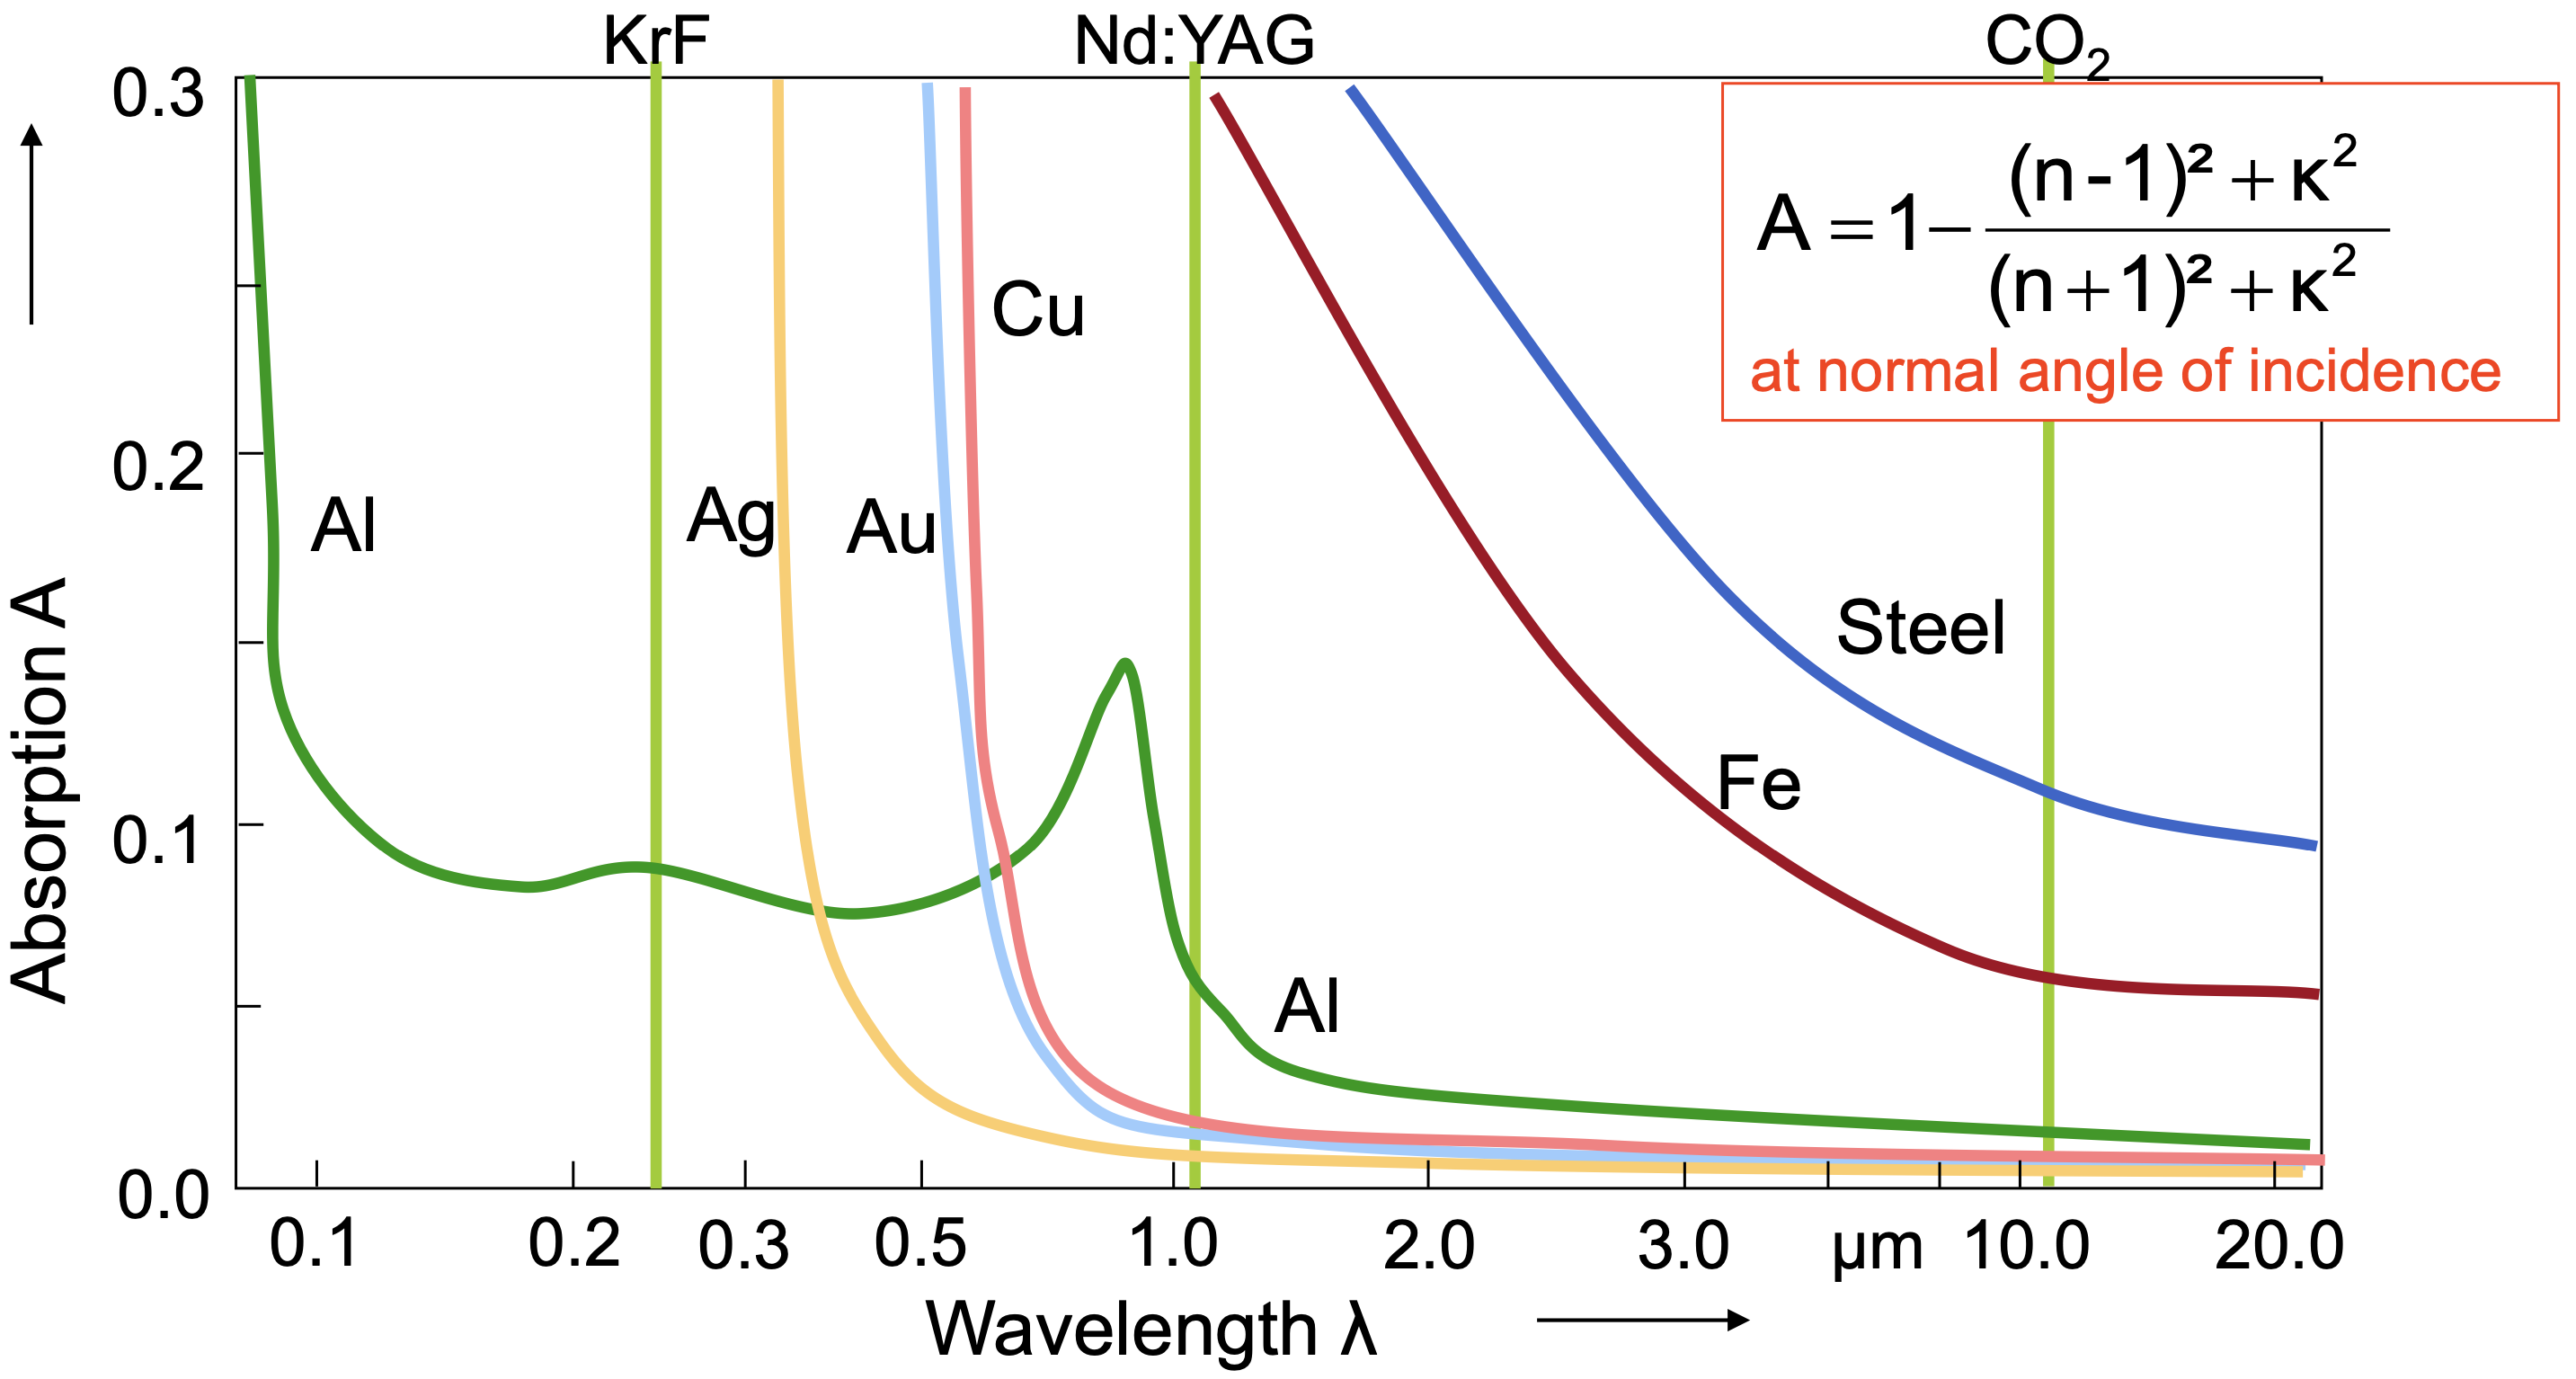
\includegraphics[width=0.5\textwidth]{slike/arwl.png}
    \caption{Absorbance of different materials at normal angle of incidence. \textit{Source:Lecture Notes.}}
    \label{fig:arwl}
\end{figure}

In general metals have high absorption rate in the UV range, low absorption rate in the visible and infrared spectrum.
Insulators have high absorption rate in UV and FIR, low absorption in VIS and NIR. Show in figure \ref{fig:tanai}.
Absorption and reflectivity depend on the angle of incidence. Figure \ref{fig:ma} show the reflectivity compared to angle of incidence.

\begin{figure}
    \centering
    \begin{subfigure}{0.45\textwidth}
        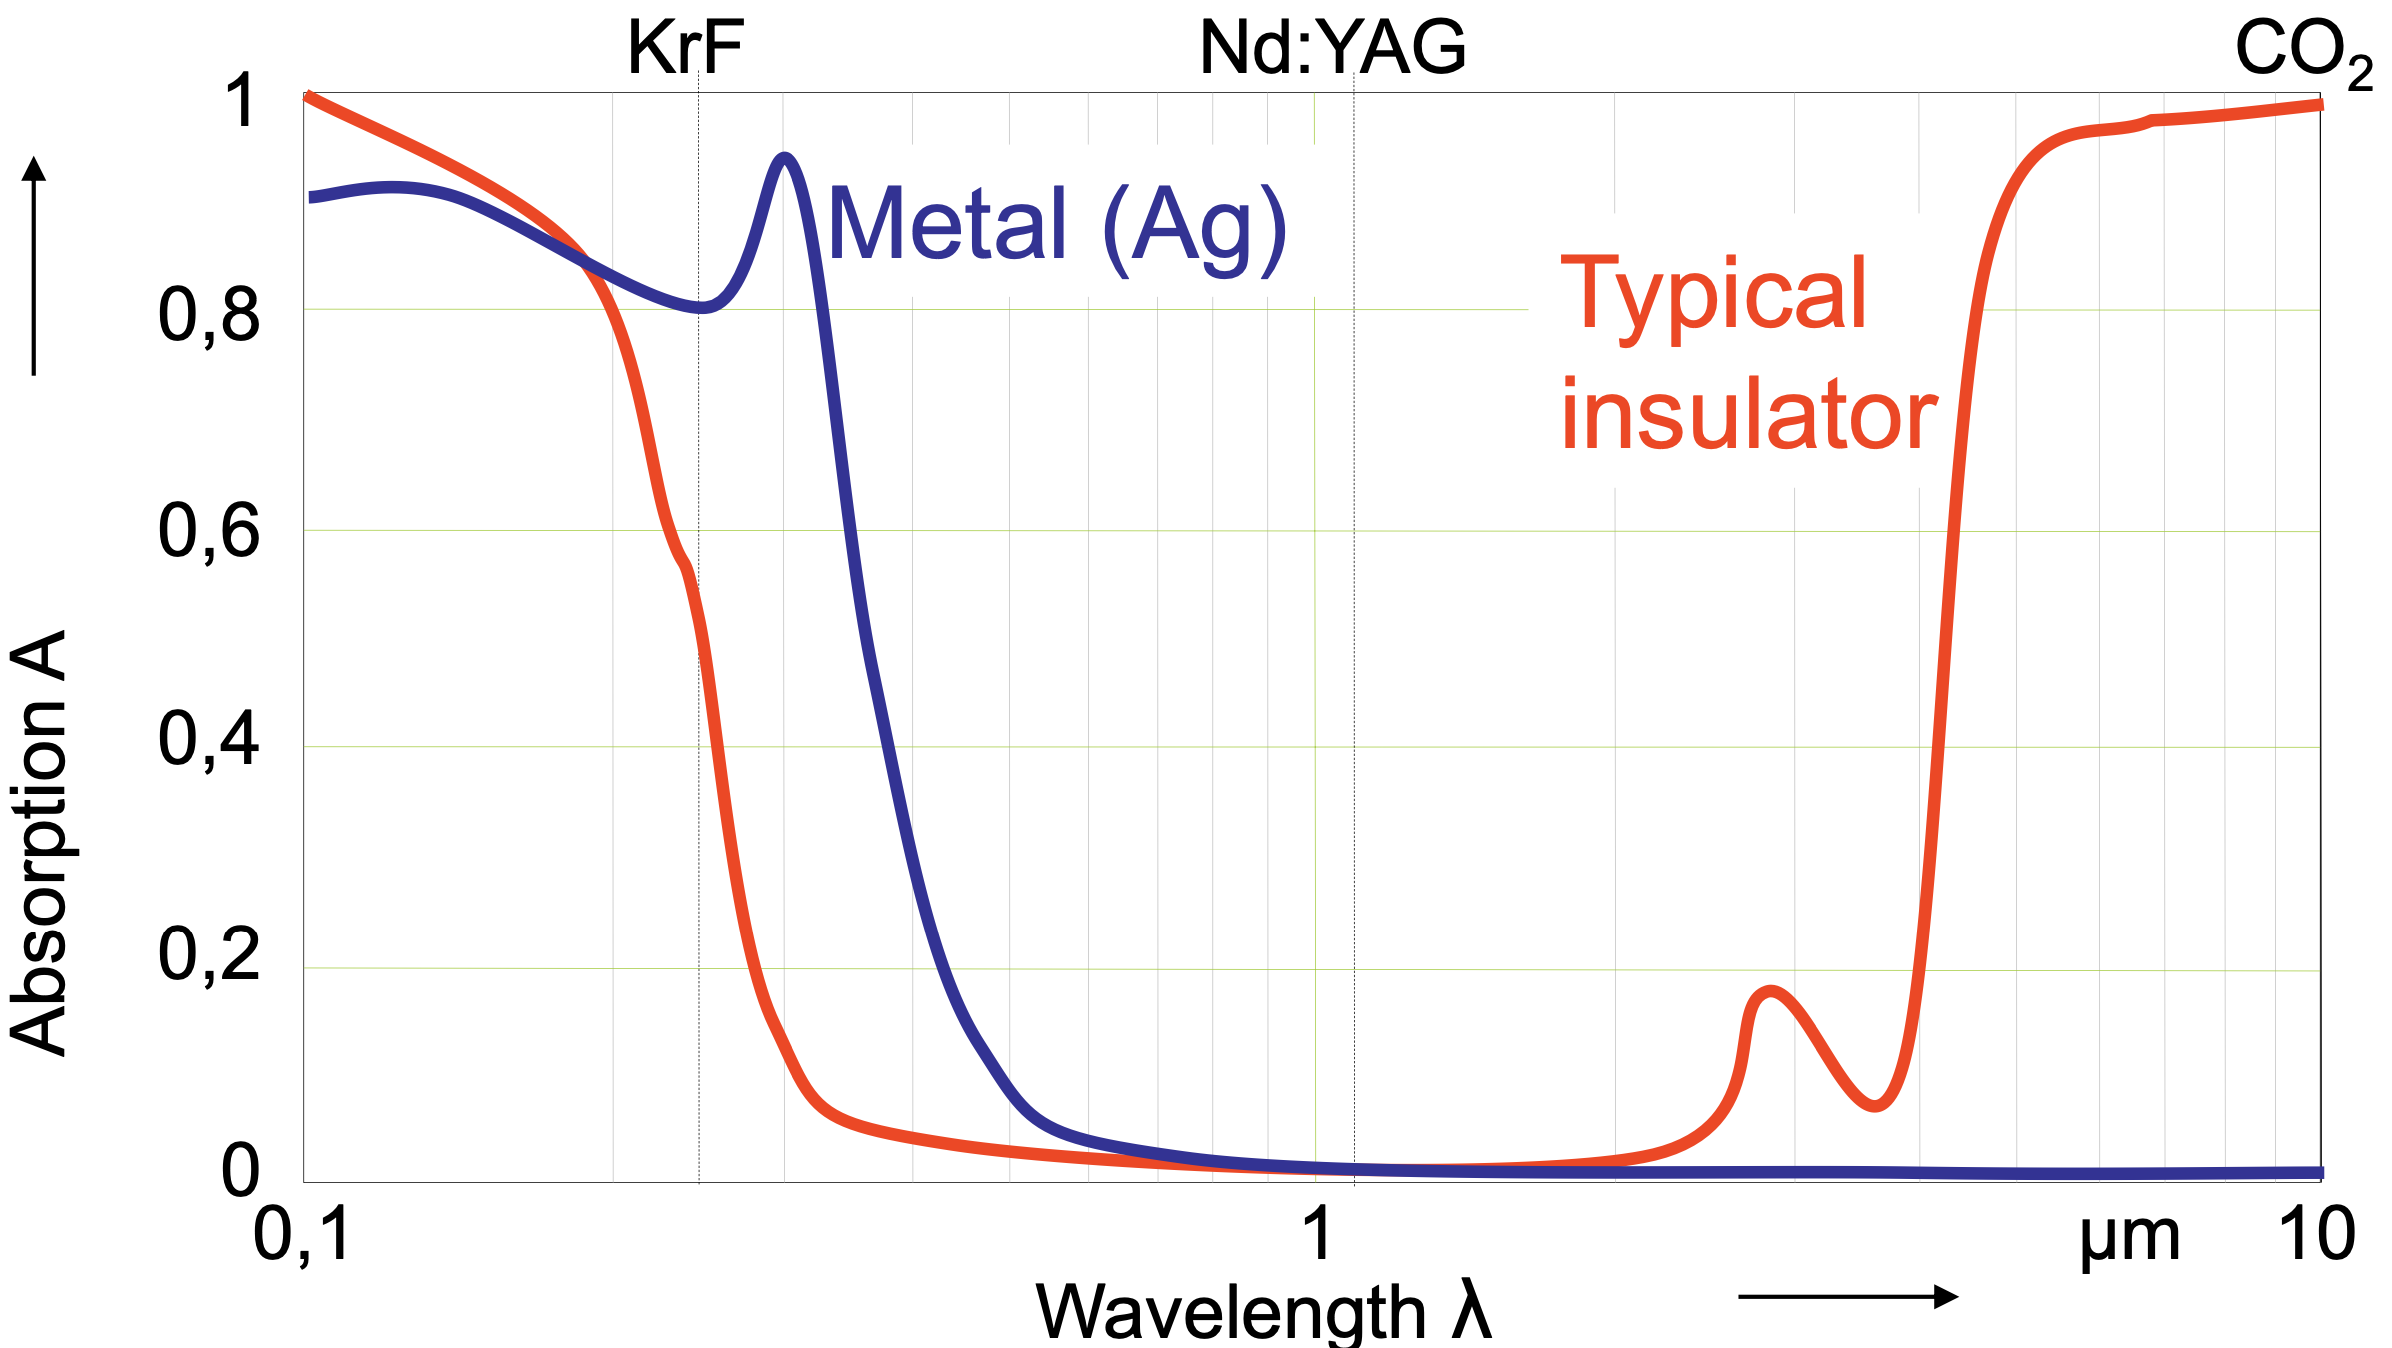
\includegraphics[width=0.45\textwidth]{slike/armi.png}
        \caption{Typical absorption curves for normal angle of incidence.}
        \label{fig:tanai}
    \end{subfigure}

    \begin{subfigure}{0.45\textwidth}
        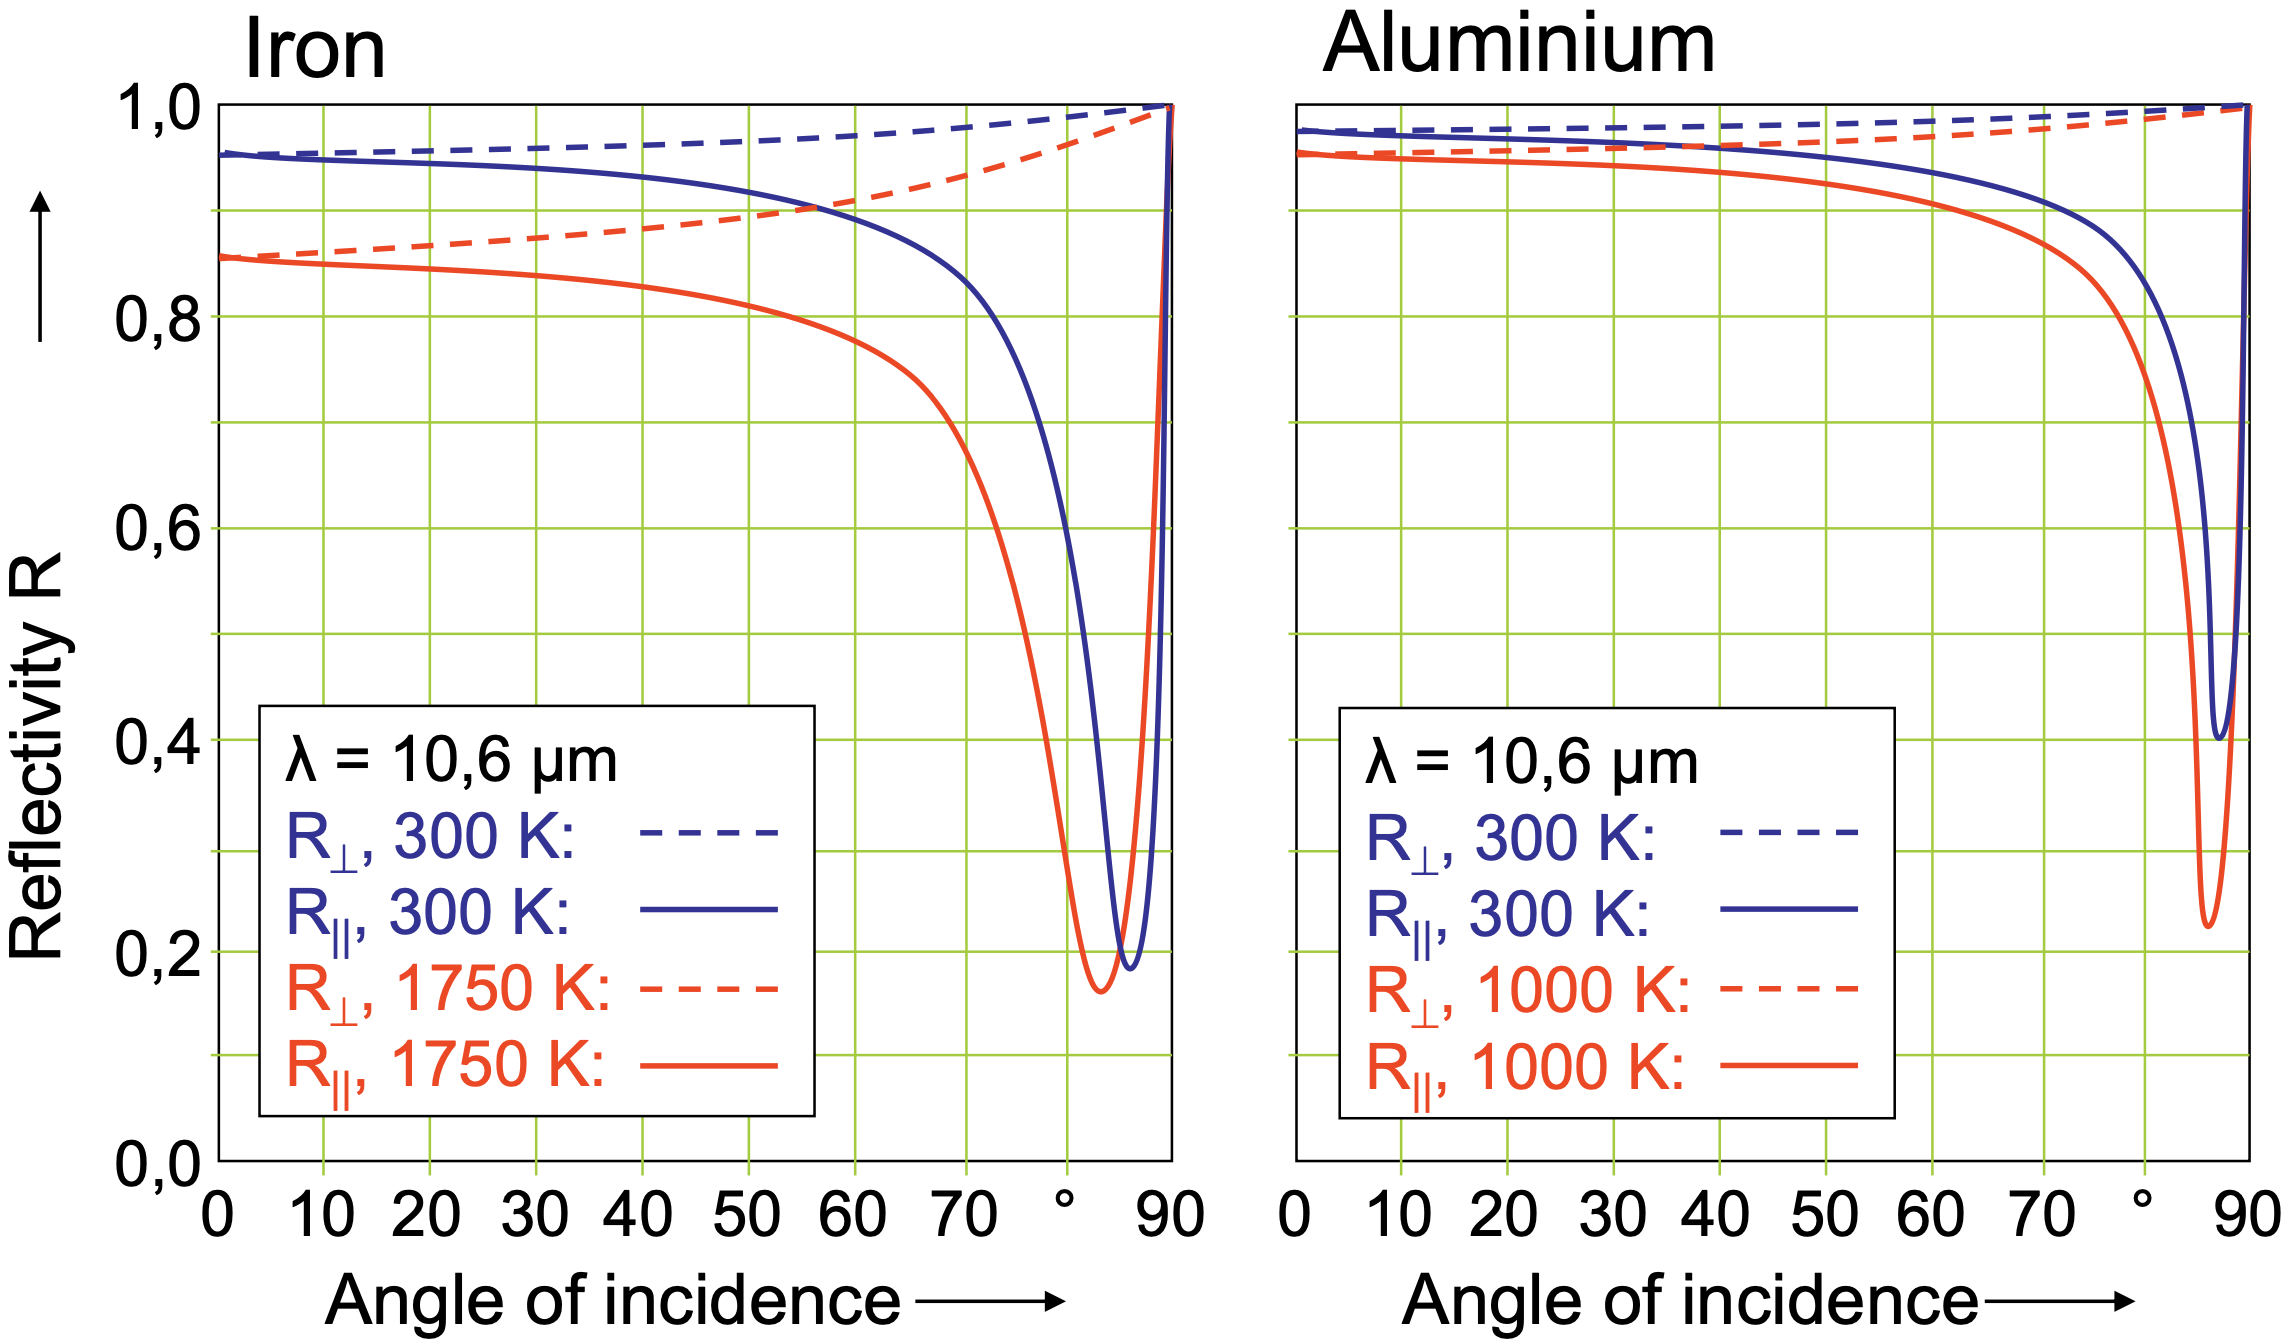
\includegraphics[width=0.45\textwidth]{slike/Rangle.png}
        \caption{Reflectivity $R$ compared to angle of incidence.}
        \label{fig:ma}    
    \end{subfigure}
\end{figure}

% \begin{figure}[h!]
%     \centering
%     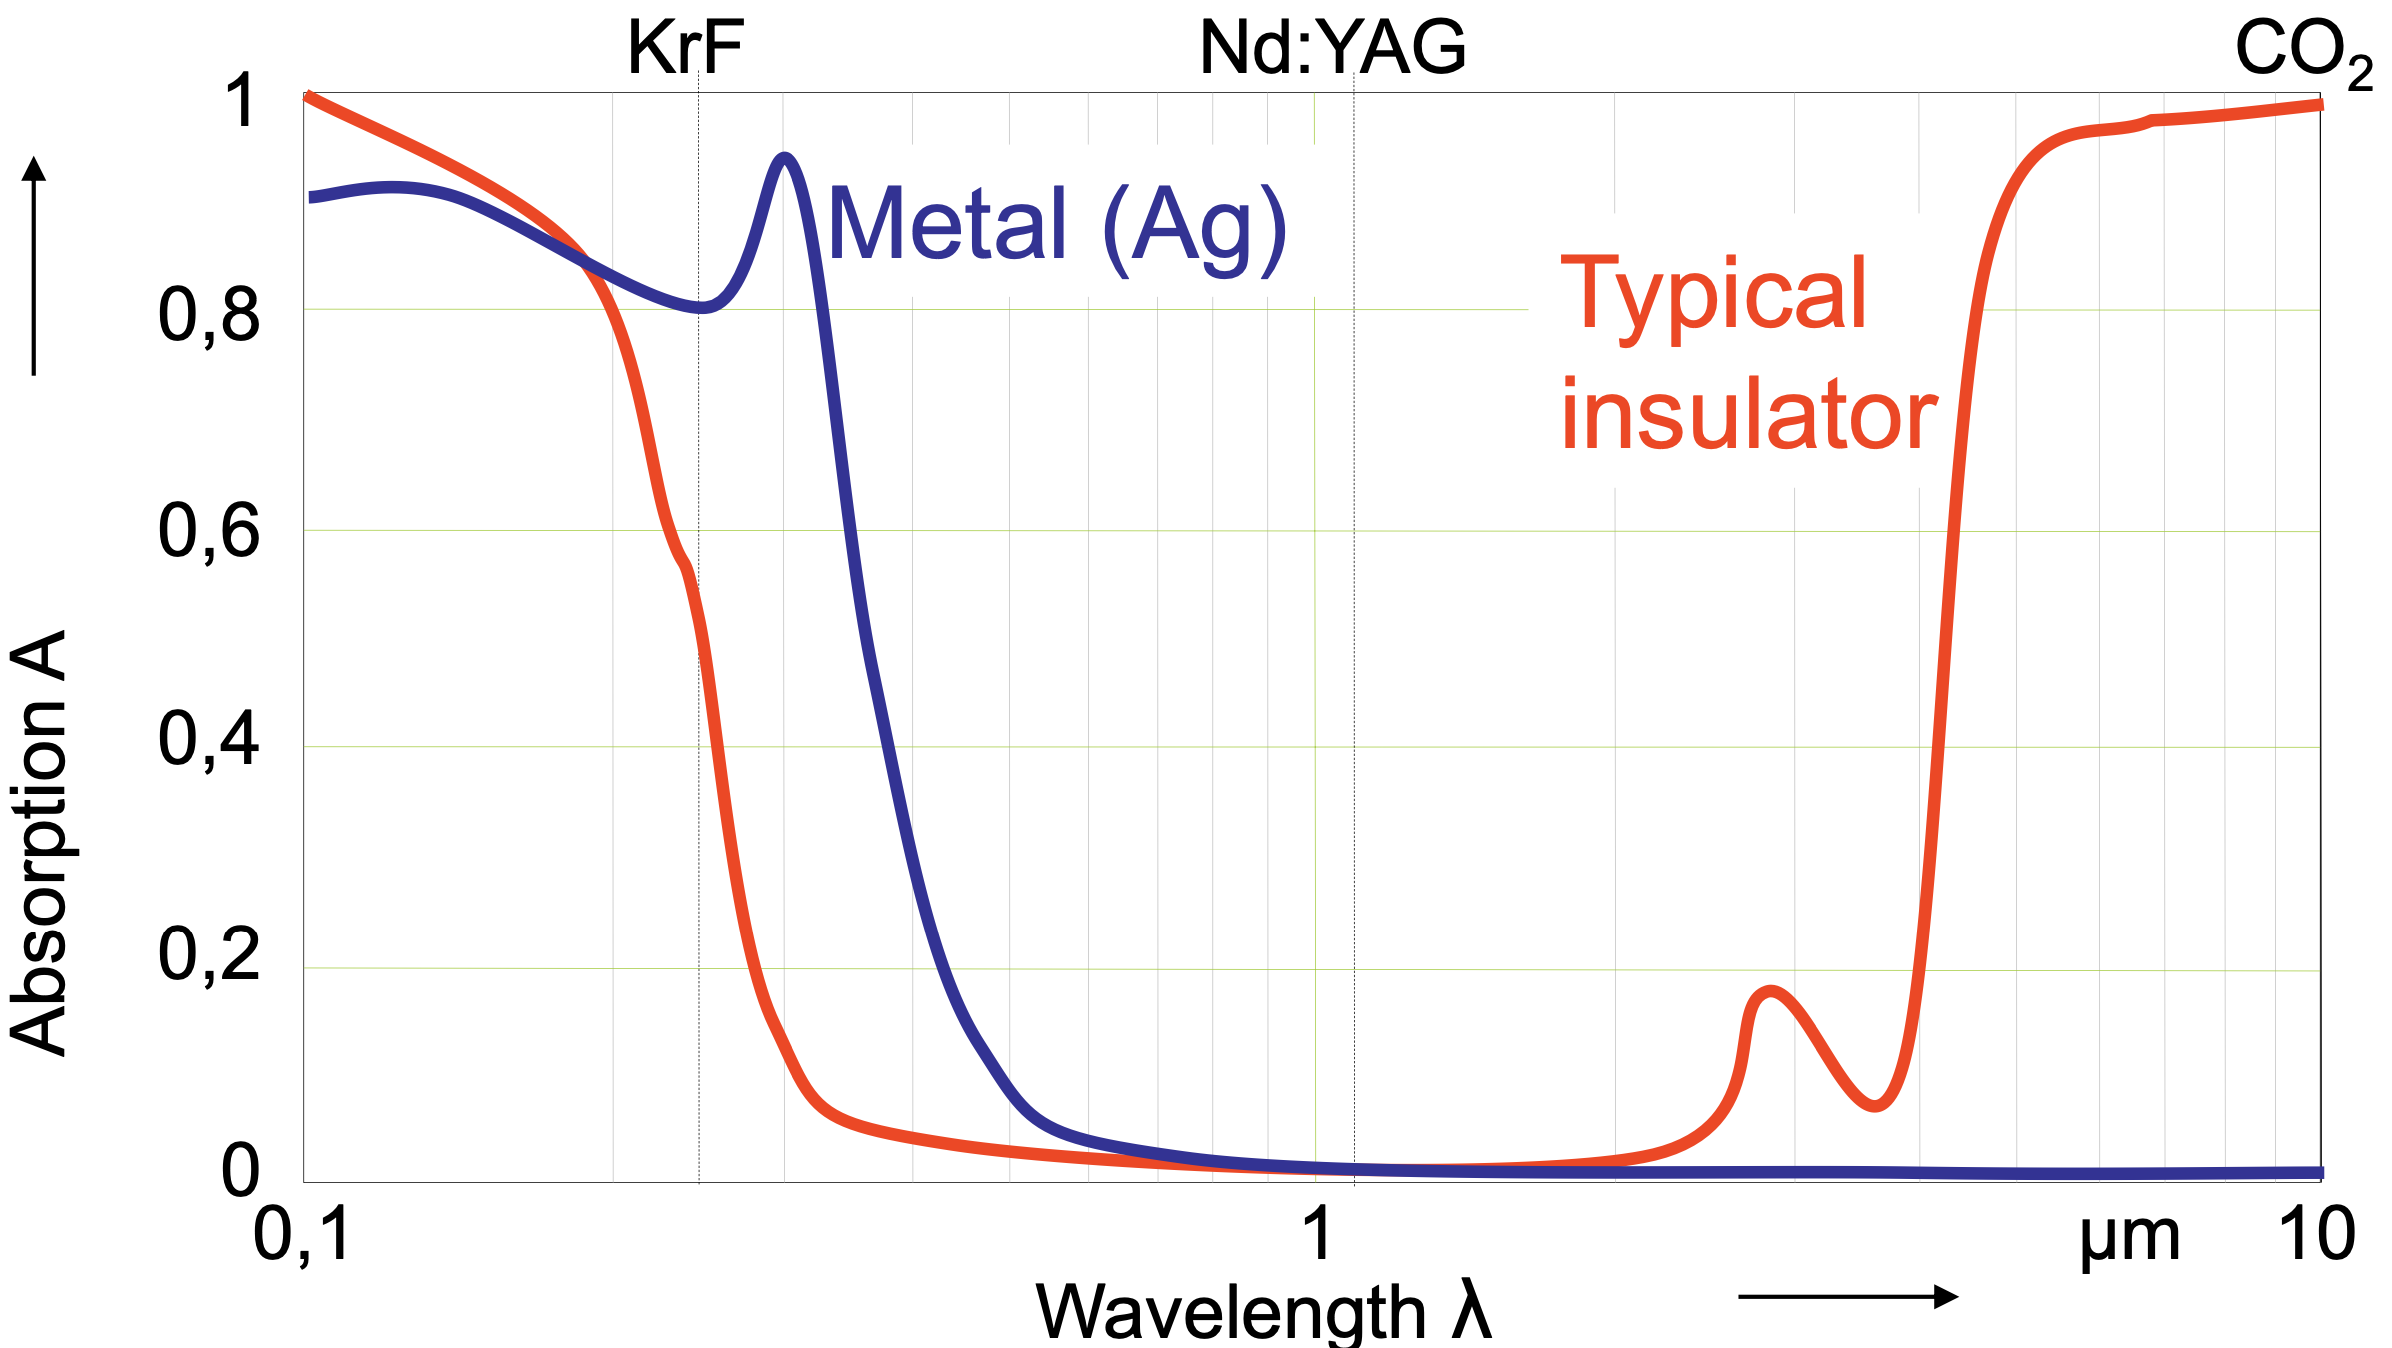
\includegraphics[width=0.5\textwidth]{slike/armi.png}
%     \caption{Typical absorption curves for normal angle of incidence. \textit{Source:Lecture Notes.}}
%     \label{fig:tanai}
% \end{figure}


% \begin{figure}[h!]
%     \centering
%     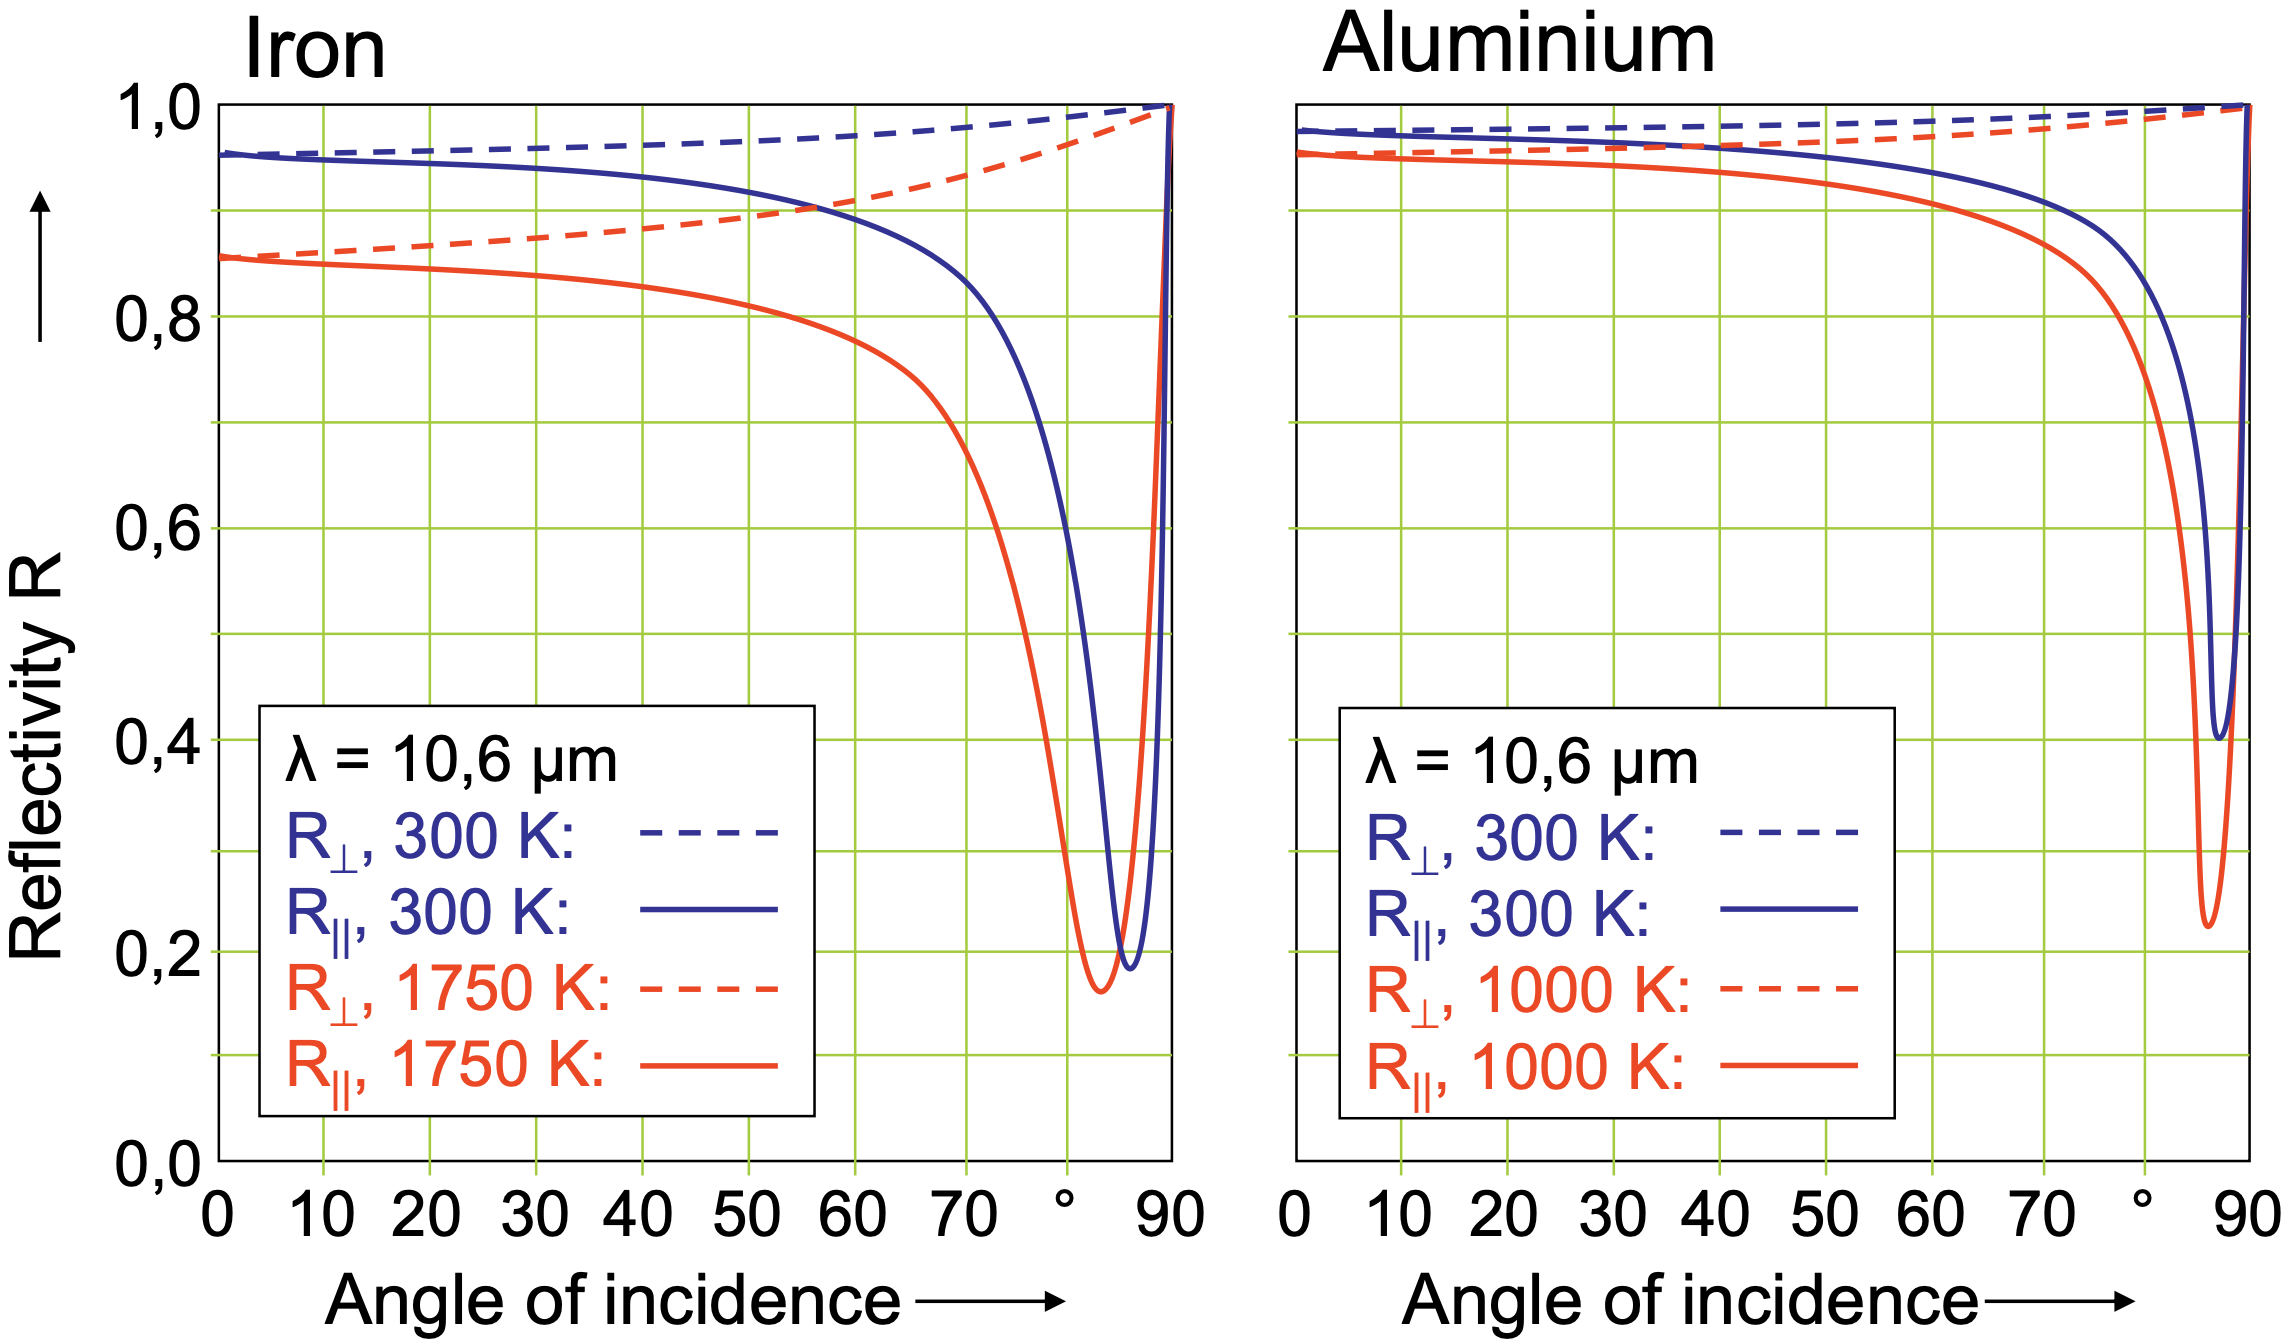
\includegraphics[width=0.5\textwidth]{slike/Rangle.png}
%     \caption{Reflectivity $R$ compared to angle of incidence. \textit{Source:Lecture Notes.}}
%     \label{fig:ma}    
% \end{figure}


\section{Rate of energy input}
Rate of energy input $\frac{\Delta E}{\Delta t}$ determines what kind of reaction light and material are going to have:
\begin{itemize}
    \item Low energy rate input \pd heating, melting, vaporization, thermal ionization
    \item High energy rate input (short and ultra short pulses) \pd MPA, MPI, direct photon dissociation of compounds, molecules \dots
    \item Low density plasma \pd highly absorbing \pd avalanche ionization
\end{itemize}

In \textbf{metals}:
\begin{itemize}
    \item Plasma interaction \pd Joule heating
    \item Thermalization rate of electrons to lattice temperature \pd \textit{nanoseconds} $\approx$ immediately.
\end{itemize}

\section{Heat effects due to laser irradiation}
Heat effect on materials depends on intensity of lasers. 
Table \ref{tab:hef} and figure \ref{fig:hef} shows intensity and processes.

\begin{table}[h!]
    \begin{tabular}{|c|c|}
        \hline
        Intensity & Process \\
        \hline
        $I \le 10^5 \frac{W}{cm^2} $ & Annealing, forming, labelling (annealing colours) \\

        $I \ge 10^5 \frac{W}{cm^2}$ &  Cutting, heat conduction welding, fusion cutting, laser sintering\\
        
        $I \ge 10^6 \frac{W}{cm^2}$ & High performance cutting, keyhole (deep penetration) welding\\
        \hline
    \end{tabular}
    \caption{Intensity of certain processes}
    \label{tab:hef}
\end{table}
%488
\begin{figure}[h!]
    \centering
    \begin{subfigure}{0.25\textwidth}
        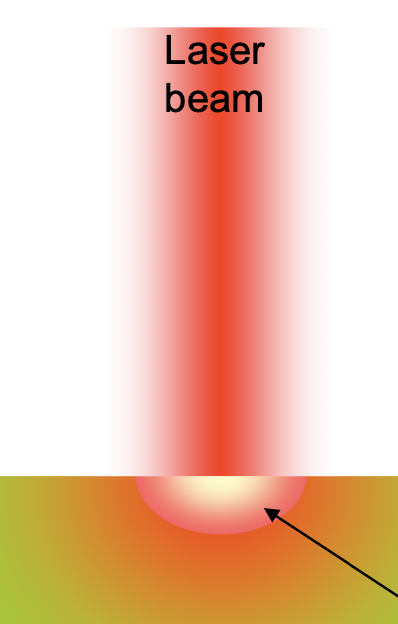
\includegraphics[width=0.45\textwidth]{slike/hef1.png}
        \caption{$I \le 10^5 \frac{W}{cm^2} $}
        \label{fig:hef1}
    \end{subfigure}

    \begin{subfigure}{0.25\textwidth}
        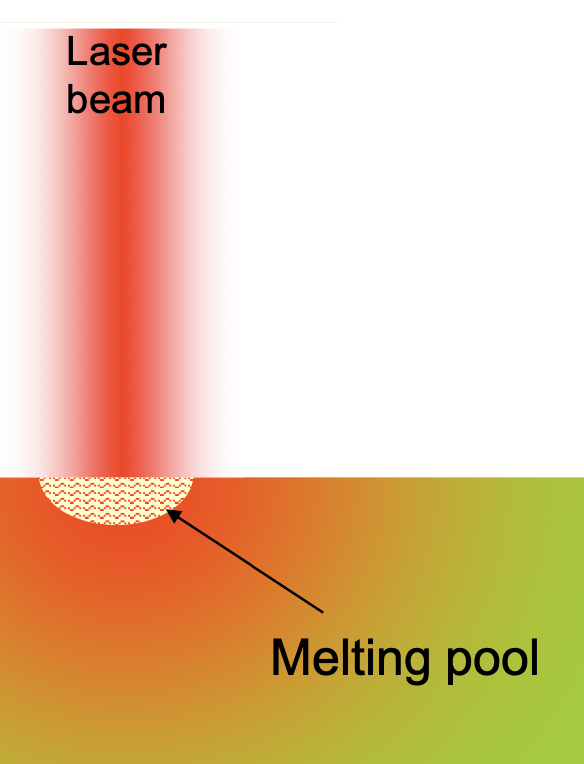
\includegraphics[width=0.45\textwidth]{slike/hef2.png}
        \caption{$I \ge 10^5 \frac{W}{cm^2}$}
        \label{fig:hef2}
    \end{subfigure}

    \begin{subfigure}{0.25\textwidth}
        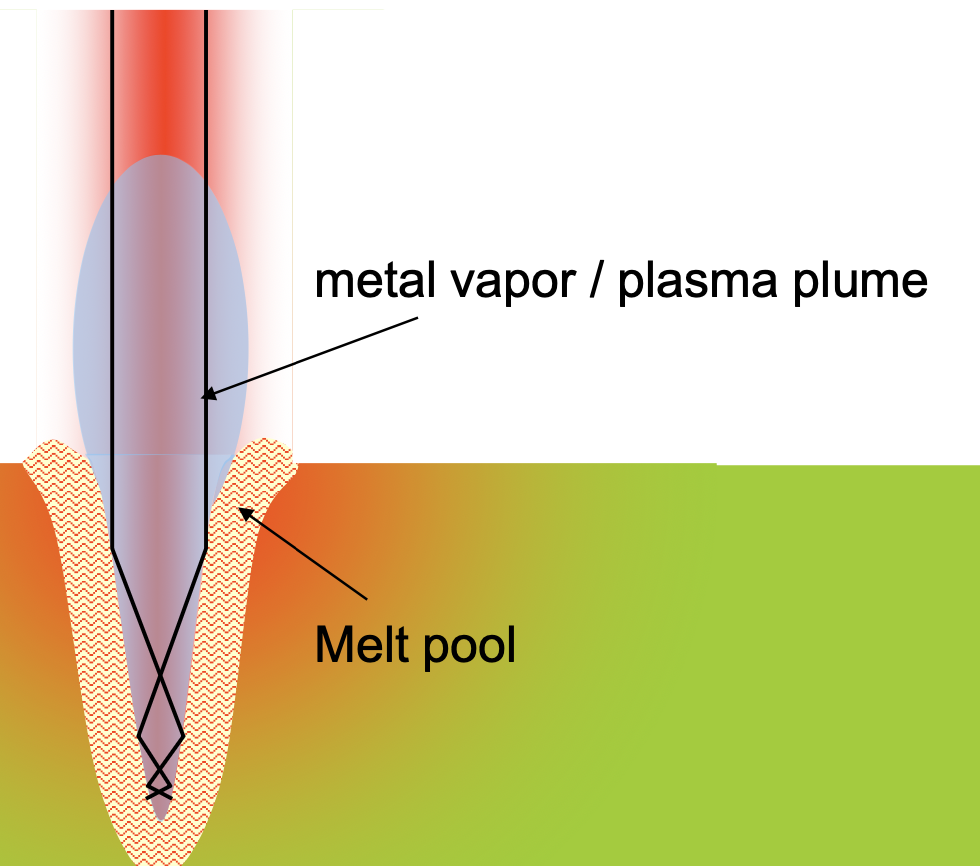
\includegraphics[width=0.45\textwidth]{slike/hef3.png}
        \caption{$I \ge 10^6 \frac{W}{cm^2}$}
        \label{fig:hef3}    
    \end{subfigure}

    \caption{Effects of heat. \textit{Source: Lecture notes.}}
    \label{fig:hef}
\end{figure}

\section{Influence of pulse duration}
Laser can have different durations of pulses. Continuous work (CW) lasers have an infinite pulse, short pulse lasers have pulse lengths measured in nanoseconds an ultra short pulse lasers have \textit{ps } and \textit{fs} length of pulses.
Processing of high bandgap materials is most effective when using MPA and MPI. Linear absorption is very ineffective. 

\begin{itemize}
    \item[] \textbf{CW-Laser} \pd hot processing:
     \begin{itemize}
        \item Low intensity \pd linear absorption required
        \item Heating, melting, evaporation, sublimation
        \item Eventual plasma generation \pd light is absorbed in the plasma (plasma density is too low for reflection)
        \item Heat generated by the laser is diffused by heat conduction, convection and thermal radiation
        \item Wide heat affected zone - HAZ \pd coarse structure
        \item[]
    \end{itemize}

    \item[] \textbf{Short pulse} \textit{ns} \pd transition from hot to cold processing
     \begin{itemize}
        \item High intensity \pd linear absorption and (thermal) plasma generation
        \item High heating rates \pd evaporation and sublimation
        \item Heat escapes by convection
        \item Smaller HAZ \pd finer structure
        \item[] 
     \end{itemize}

     \item[] \textbf{Ultra short pulse} \textit{ps,fs} \pd cold processing
     \begin{itemize}
        \item Extreme intensity \pd immediate plasma generation, electron gas temperatures \pd fast thermalization
        \item Columb explosion \pd Plasma explosion
        \item Heat removal with plasma explosion \pd fast heat removal
        \item Almost no HAZ \pd very fine structure
        \item[]
     \end{itemize}
\end{itemize}

%500

\textbf{Heat affected zone - HAZ} is the part of material whose structure effected by heat. Even for short and ultrashort 
pulses (\textit{ns, ps, fs}) pulses have to be timed to prevent heat accumulation. Show in figure \ref{fig:ptiming}.
\begin{figure}[h!]
    \centering
    \includegraphics[width=0.5\textwidth]{slike/tpulses.pdf}
    \caption{Pulse and cooldown}
    \label{fig:ptiming}
\end{figure}


At high repetition rates residual heat will accumulate - high temperatures can be reached, which can be useful for glass or silver welding.
Shown on figure \ref{fig:usprr}.

\begin{figure}[h!]
    \centering
    \includegraphics[width=0.75\textwidth]{slike/prepet.pdf}
    \caption{Ultra short pules with fast repetition. \textit{Source: Lecture notes.}}
    \label{fig:usprr}
\end{figure}

Secondary effects of this are \textbf{Incubation effects}.
If the energy of single pulse is too low for ablation or visible material modification material properties can still be changed be the laser radiation.
Effect of this can be \textit{partial oxidization} which causes strong changes of absorptivity. Impurities and lattice (structural) defects have much lower 
bandgap than the rest of material and can still get excited into meta stable states - we still do not see any obvious material modification.
When a high enough population of excited defects is reached, material processing becomes possible.
Incubation is observable in metals and insulators.


